% !TEX root = arbeit.tex
\section{Theory}
	Add a Chapter about electric fields?/ Basis for the simulations?
	\subsection{Requirements}
	% Mass, performance, Power consumption. (See latest references. Part of the introduction?)
	
	\subsection{Basic Theory about TOF Masspectrometry} % Allgemeine Theorie
	
	% Priciples kann immernoch weiter ausgearbeitet werden falls nötig.
	\subsubsection{Principle} % Noch Referenzen auf Vorlesung einfügen. Evt. noch Bild eifügen von Ionen an versch. Startpositionen.
	This chapter explains the function of a TOF instruments. A TOF mass spectrometer consists of, an ion-source, a mass analyser and a detector. The mass analyser has an ion-mirror which increases the flight distance of the ions by keeping the instrument on a certain length. A longer flight distance increases the mass resolution of the instrument.\\% Mention that later.
	In the ion source, the ions are produced. An electric field in the source is generated such that ions get trapped in it. Then ions get accelerated by applying a high voltage pulse on the extraction grid. \textcolor{red}{Include a Graphic of the IS and draw a sample electric field to explain how the extraction pulse (the door to open) works.}
	If the pulse width is long enough that all ions leave the source during the time the pulse is applied, the ions get all the same amount of energy $W$
	\begin{equation}
		W = \int_{0}^{s_0}q_0 E_s ds = q_0 U_0
	\end{equation}
	With $s_0$ the distance the ions get accelerated, in our case 1\si{\milli\metre} which is half the height of the ion source, $q_0$ the elementary charge, $E_s$ the applied electric field strength and $U_0$ the voltage applied on the extraction grid. This energy is equal to the kinetic energy the ions have after leaving the ion-source
	\begin{equation}
		q_0 U_0 = \frac{1}{2}m v^2
	\end{equation}
	With $m$ the mass of the particle and $v$ the particle velocity. Rearranging this formula we get
	\begin{equation}
		\frac{m}{q_0} = 2 U_0\frac{t^2}{s^2}
		\label{eq:m/q}
	\end{equation}
	With $t$ the time of flight and $s$ the flight distance. Therefore, $m/q_0$ is proportional to $t^2$.\\
	Ions starting at different positions also get a different amount of energy. Ions starting closer to the extraction grid will get less energy than ions further away from the grid. At a certain point after the source, the ions with higher energy have overtaken the slower ions. This point is at around $2\cdot s_0$ which corresponds to a very short flight distance. To shift this focal point onto to the detector, additional fields after the ion-source are applied.\\
	The ions have different thermal energies. Therefore ions of the same mass and the the same starting position will not have all the same energy when they leave the ion source. This energy spread leads to a difference in their velocity and to different flight times. This energy spread can be partially compensated by an ion-mirror also referred to as reflectron (Fig.\,\ref{fig:NIMSketch}). Ions with a higher energy will penetrate deeper into the ion-mirror and have a bigger flight path than ions with less energy. Therefore, the ion-mirror is able to compensate the different start energies of the ions. In the worst case scenario we have one particle flying toward the extraction grid and the other particle flying with the same velocity in the opposite direction. The second particle gets decelerated and has to turn in the source. When it reached its initial position, it has the same amount of energy as the first particle. But it will always be behind the first particle by a constant time delay needed to turn around and reach its initial position. To minimize this effect, one has to minimise the distance of the ionisation region or increase the voltage of the HV pulse. A smaller ion source means less ions and therefore less signal. Increasing the HV pulse results in bigger electronic noise at the start of the spectrum and fast species such as hydrogen of helium are lost in the noise. % Evt. noch Effekte etwas besser ausführen.

	\subsubsection{Mass Calibration}
	In this section we discuss the calibration of the mass axis. According to Eq.\,\eqref{eq:m/q} the $m/q_0$ is proportional to the square of time. By rearranging Eq.\,\eqref{eq:m/q} $m$ is:
	\begin{equation}
		m = 2 q_0 U_0 \frac{t^2}{s^2}
		\label{eq:mass_Calib_pre}
	\end{equation}
	Take together all parameters which remain constant to one single constant: % Write a bit better
	\begin{equation}
		C = \frac{2 q_0 U_0 }{s^2} 
	\end{equation}
	and considering the time scale has a constant offset $t_0$, equation \eqref{eq:mass_Calib_pre} results in % Split the two ts. It is not acctually the same.
	\begin{equation}
		m = C(t-t_0)^2
		\label{eq:mass_Calib}
	\end{equation}
	In this equation there are two free parameters, $C$ and $t_0$. To calibrate a mass spectrum at least two species appearing in the spectrum have to be known to solve this equation for the two parameters.
	% [Scherer 1999]
	
	\subsubsection{Mass resolution} % Bild einfügen, wie die Mass Resolution berechnet wird.
	The mass resolution is calculated as follows. According to Eq.\ref{eq:mass_Calib} $m$ is:
	\begin{align*}
		m &= c\cdot t^2\\
		\frac{dm}{dt} &= 2ct\\
		dm &= 2ct\cdot dt\\
		\frac{m}{dm} &= \frac{ct^2}{2ct\cdot dt}
	\end{align*}
	% Source down to here is from the lecture.
	Resulting in:
	\begin{equation}
		\frac{m}{\Delta m} = \frac{t}{2 \Delta t} = \frac{\mu_t}{2 FWHM_t}
		\label{eq:mass_res}
	\end{equation}
	With $\mu_t$ the centre of the mass peak in the time domain and $FWHM_t$ the full width at half maximum. The $FWHM_t$ depends on several parameters. For example the turn around time of the particles, the energy spread resulting from different starting positions of the particles relative to the extraction grid, spread in thermal energy. The reflectron is able to compensate for the energy spread by a certain amount. % Maybe explain that a bit further
	There are also limitations of the instrument itself. For example the performance of the pulser which will be discussed later in Chap. bla.
	\begin{comment}
		Resolution limitations:
		Pulser:
		Turn around time
		Different starting positions (discussed a little bit further above)
		Reflectron: Not ideal energy focusing -> spread
		Thermic energy -> spread
		instrument limitations: not perfect pulser pulse. discussion of Pulser follows maybe a bit later.
		peak width of the single ions measured with the detector. Peak width of 1 peak is b< a factor 10 smaller than the actual peak in the mass spectrum.
	\end{comment}
	% Mass resolution is independant from the actual mass
	% Last part of the formula is from Stefans thesis.
	
	% Then continue with the calculation of the mass resolution and the calibration of the mass scale (evt. Reference further explanation how the software it acctually does (keep it short, only extend it if further nessecary)).
		
	\subsubsection{Signal-to-Noise Ratio and Sensitivity}
	
	\textbf{SNR}\\ % Write a bit more detailed. What does background corrected mean? Subtraction of the baseline if it is elevated.
	The SNR is defined as the ratio of the background corrected peak amplitude $I^{max}_P$ and the standard deviation of the base line $std(I_b)$ \cite{Agilent_TechNote_SNR}, \cite{Master_Meyer}: % Thechnical Note Agilent and Masterarbeit Stefan.
	\begin{equation}
		SNR = \frac{I^{max}_P}{std(I_b)}
		\label{eq:SNR}
	\end{equation}
	A high mass resolution improves also the signal-to-noise ratio. By better focusing the ions in the time frame, the peak gets narrower. The area under the peak corresponds to the number of ions. If the number of ions and therefore the area under the curve stays the same, a narrower peak implicates an increase in signal height and therefore in a higher SNR.\\ % In other mass spectrometers (such as sector magnets) an increase in mass resolution results in a reduction of the phase space and therefore in a loss of signal intensity.
	\\
	\textbf{Sensitivity} \\ % Really include this chapter? Because it is only an estimation of the actual performance of the instrument. If it is included, do a proper derivation of the formula!!
	The sensitivity $n_{lim}$ is the actual detection limit of the sensor. It is defined as the amount of gas detected by the instrument $n_{det}$ over the amount of ions entering the instrument $n_{p}$ times the signal intensity measured by the instrument $I_{sig}$
	\begin{equation}
		n_{lim} = \frac{n_p \cdot I_{sig}}{n_{det}}
	\end{equation}
	
	
	\begin{comment}
		SNR
		[Wells 2011]
	\end{comment}
	
	\begin{comment}
		Sensitivity
		
	\end{comment}
	
	% SNR, Sensitivity
	
	% Uncertainty cause by the 'Umkehrzeit'. Distance between 2 and 3 is always the same and depends on Uth
	
	% Include a schematics of the ion source with the different states/ effects.	


	
	\subsection{Ion Optical Design, NIM specific elements} % Inspiration from the arguments of the paper. Titel noch anpassen. Theorieteil fortlaufend hinzufügen. Ion source efficienies, reflectron double focusing, detector reflection of signal, signal matching. Density enhancement.
	% Hier das Design allgemein halten. Erst in Kapitel 'Setup' auf die Designdetails eingehen. Discuss important theory parts here and just give a short summary in the corresponding experimental parts when the theory is used.
	
	A time of flight mass spectrometer consists of, an ion-source, a mass analyser and a detector.\\
	
	\begin{figure}[htb] % Noch schauen, ob das noch verschoben wird.
		\centering
		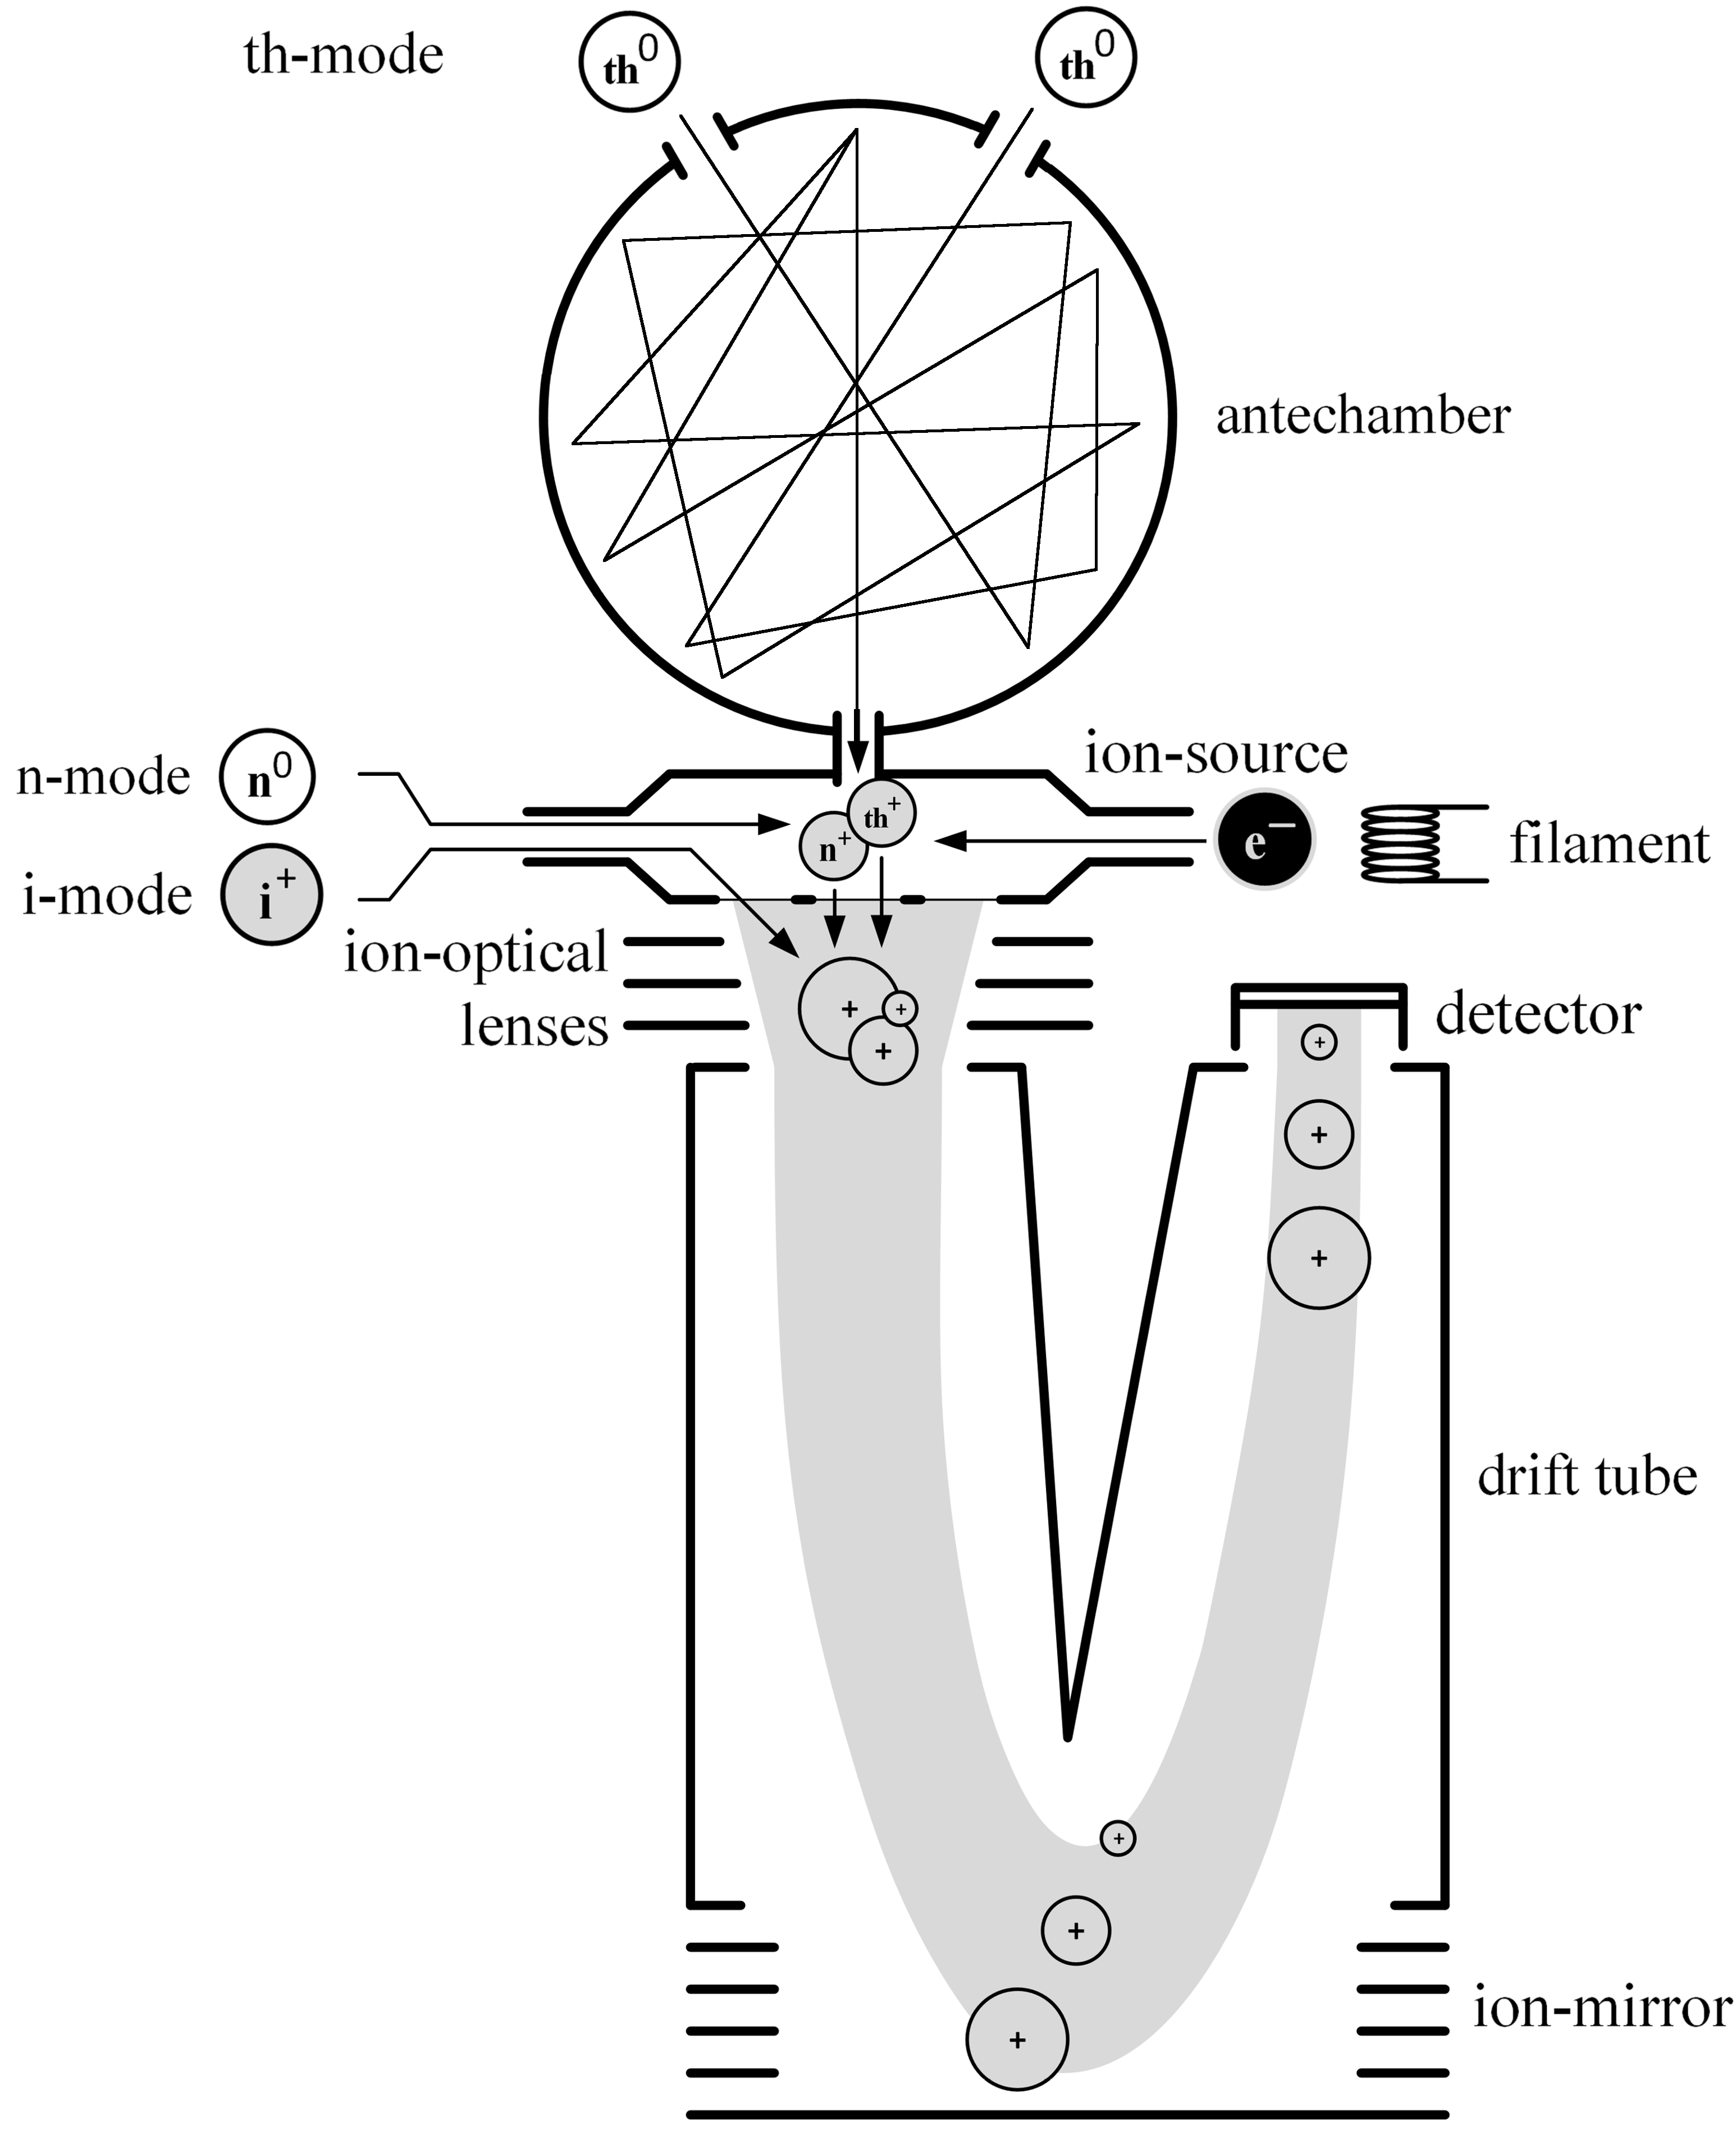
\includegraphics[width= 10cm]{Bilder/NIM_Sketch.png} % Bei Bild noch schauen, ob die Ränder drauf sind. Bei Zeiten noch Bild anpassen.
		\caption{Schematics of the NIM mass spectrometer. Adapted from \cite{Diss_Meyer}.}
		\label{fig:NIMSketch}
	\end{figure}

	%First overview and then go into the details.
	The NIM instrument is able to measure neutrals and ions. Neutral particles get ionised by electron ionisation. A filament is heated up until it emits electron. Ions enter the ion source directly.  % Noch genaue Formulierung nachschauen.
	All ions then get accelerated to the same energy and fly through the mass analyser. Light particles fly faster through the spectrometer than heavier ones. The different particle species arrive at different times at the detector. To enlarge the flight distance, an ion-mirror, which reflects the ions and leads them back to the detector. The used detector is a MCP detector. % Explain a little bit in more detail.
	
		\subsubsection{Ion Storage capability}
		% Take arguments from the paper + after a certain time, the space charge of the ions overcomes the trapping potential of the electron beam. At this point, the ions are no longer holded by the potential and leak out of the ion-source. Add space charge calculation.
		
	
		\subsubsection{Peak Analysis Statistics}
		% See notes from the paper and make a detailed Analysis/ description of the method.
		% A/mbar alias A/ #cm^3 is a instrument specific constant. Determine it for NIM.
		
		\subsubsection{Pressure calibration of the NIM Sensor}
		% More detailed explanation about the NIM ion source, function of the different specific electrodes. Or explain it later in detail when discussing the simulations in detail. See paper as a guide line. Especially for the ion storage part.
		
		To calculate the number of ions produced in the ion source we use:
		\begin{equation}
		I_{ion} = \beta\cdot Q_{ion}\cdot L\cdot n\cdot I_{em}
		\end{equation}
		With $\beta$ the extraction efficiency which is 1, % Noch schauen auf welchen Wert wir diese setzen wollen. 1= sehr gute Quelle, 0.01 = 1mus/100mus = Pulslänge Pulser/ Länge 1 Zyklus. Noch diskutieren, welche Werte beta haben kann oder einfach etwas setzen? Da die ersten Messresultate gut sind, würde ich eher auf 1 setzen. Abschätzung? Auf Unterschiede beim Spannungsset hinweisen -> beeinflusst beta massgeblich.
		$L$ as the effective ionising path in our case 4~\si{\milli\metre}, $n$ the particle density, $I_{em}$ the electron emission current from the filament and $Q_{ion}$ the ionising cross section. The cross sections of species used in our calibration can be found in table % Ref. auf Tabelle und nur auf Stefans Diss verweisen oder die 4 Originalpaper zusammen suchen. Tabelle einfügen.
		
		\subsubsection{Filament Power Calculation}
		
		
		\subsubsection{Detector Gain}
		% Explain as far as it is needed for the analysis of the detector results. Predictions, extrapolations on how the detector UMCP depends on UStack. Have a look on how big this calculation is and may put it to the detector results in the experiments chapter.
		


		
		% Reference: Bieler Diss 2012, Wurz 2011, Scherer 1999, Meyer 2013 Data Analysis, Wells 2011
		% Ionisation efficiency
		% Description of how it works with the energies. Electric -> kinetic. Pulser. E = 1/2 mv^2 = qU
		% Time focusing?
		% Mass calibration t/dt -> m/dm.
		% SNR definition. Picture?
		% Sensitivity estimation. Nessesary? If so, part of SNR discussion.
		% MCP detector. Gain calculation. How the detecotr works. Didn't do anything for further developement...
		% Antchamber. Explanation of closed and open source. Field of view. Densitiy enhancement.
	
	
\begin{comment}
	
	Explain how a TOF works. Source, reflectron, detector.
	Explanation of the antechamber at the end after explaining the different parts.
	
	Detection efficiency Ionsource, MCP? -> y-Achse
	Mass Analyser, mass spectrometer. Most important formulas. dm/m = dt/t...
	Sensitivity
	Density enhancement -> explanation about closed and open source
	Sketch of the instrument
	Requirements: Power, mass, mass resolution,... (At the end or at the beginning. Introduction)
	
	
	Ionisationseffizienz/ Ionenproduktion der wichtigsten Gase. Detektionseffizienz hängt auch von Effizienz der MCPs ab... Erklären weshalb man die Achsenskalieruing braucht (entweder Counts oder die angepasste a.u. bei der Fläche und Counts/s für das Spektrum)
	
\end{comment}
		